%\documentclass{article}
%\usepackage[utf8]{inputenc}
%\usepackage{tikz}
%\usetikzlibrary{positioning}
%\begin{document}
	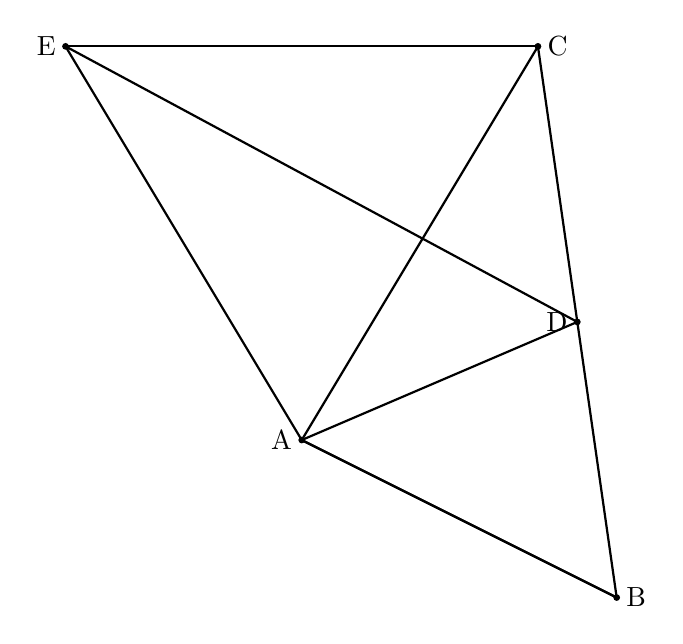
\begin{tikzpicture}
		\draw[black, thick] (0,0) --(4,-2); 
		\draw[black, thick] (4,-2)--(3,5);
		\draw[black, thick] (3,5)--(-3,5);
		\draw[black, thick] (-3,5)--(0,0);
		\draw[black, thick] (0,0)--(3.5,1.5);
		\draw[black, thick] (0,0)--(4,-2);
		\draw[black, thick] (0,0)--(3,5);
		\draw[black, thick] (3.5,1.5)--(-3,5);
		
		\filldraw[black] (0,0) circle (1pt) node[anchor=east] {A};
		\filldraw[black] (4,-2) circle (1pt) 
node[anchor=west] {B};
		\filldraw[black] (3,5) circle (1pt) node[anchor=west] {C};
		\filldraw[black] (-3,5) circle (1pt) node[anchor=east] {E};
		\filldraw[black] (3.5,1.5) circle (1pt)
node[anchor=east] {D};
	\end{tikzpicture}
%\end{document}